% begin module infinite-limit-ln-tan
\begin{frame}
\begin{columns}
\column{.5\textwidth}

\psset{xunit=1cm, yunit=1cm}
\begin{pspicture}(-0.1,-3)(4.6,1.9)
\psaxes[ticks=none, labels=none]{<->}(0,0)(-0.1,-3)(4.5,1.8)
\psline(1,-0.1)(1,0.1)
\rput[tl](1, -0.15){$1$}
\rput[r](-0.15,1){$1$}
\psline(-0.1,1)(0.1,1)
\rput(3, 0.6){$y=\ln x$}
\psplot[linecolor=red, plotpoints=1000]{0.048}{5}{ x ln}
\end{pspicture}
%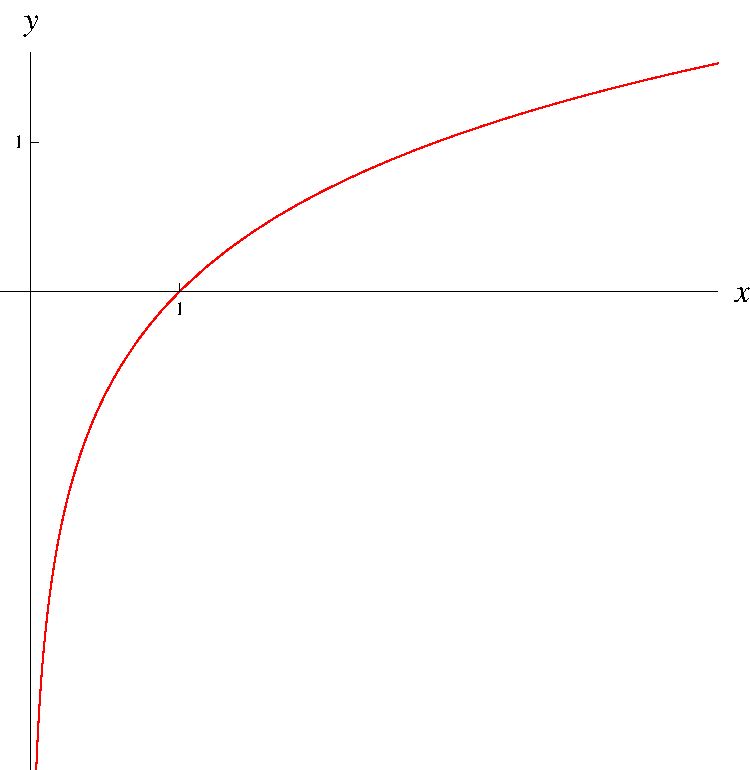
\includegraphics[width=5cm]{limits/pictures/graph-ln.pdf}


%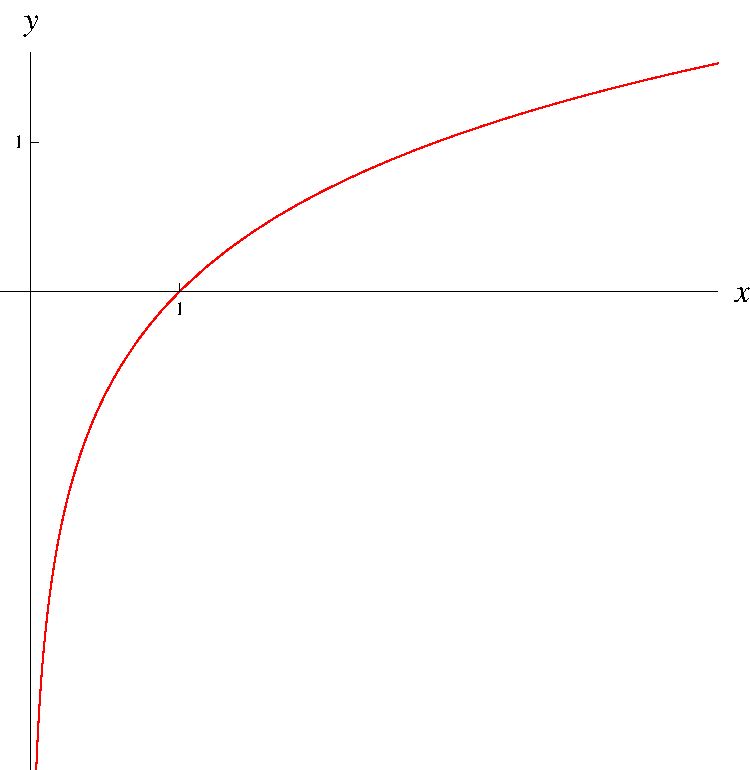
\includegraphics[width=5cm]{limits/pictures/graph-ln.pdf}

\abovedisplayskip=0pt
\belowdisplayskip=-15pt
\abovedisplayshortskip=0pt
\belowdisplayshortskip=0pt
\begin{align*}
\alertNoH{ 2-3}{\lim_{x\to 0^+}\ln x} & \alertNoH{ 2-3}{=} \fcAnswer{3}{-\infty} \\
\end{align*}
\column{.5\textwidth}

\psset{xunit=0.25cm,yunit=0.25cm}
\begin{pspicture*}(-5.5,-10)(10.6,10.1)
\psaxes[labels=none, ticks=x, Dx=1.570796327] {<->}(0,0)(-5.5,-10)(5.5,10)
\rput[lt](5.5,0){$x$}
\rput[lb](0.2,9){$y$}
%\rput[t](1,-0.1){1}
\psline[linecolor=gray](1,-0.1)(1,0.1) % x unit mark
\rput[lb](1.570796327,0.1){$\frac{\pi}2$}
\psline[linecolor=gray](1.570796327,-0.1)(1.570796327,0.1) % pi/2 unit mark
%\rput[br](0,1){1}
\psline[linecolor=gray](-0.1,1)(0.1,1) % y unit mark

\psplot[linecolor=red]{-1.57}{1.57}{ 180 x mul  3.1415 div tan}
\psplot[linecolor=red]{-4.71}{-1.58}{ 180 x mul  3.1415 div tan}
\psplot[linecolor=red]{1.58}{4.71}{ 180 x mul  3.1415 div tan}

\psline[linestyle=dotted](-4.71238898,-10)(-4.71238898,10)
\psline[linestyle=dotted](-1.570796327,-10)(-1.570796327,10)
\psline[linestyle=dotted](1.570796327,-10)(1.570796327,10)
\psline[linestyle=dotted](4.71238898,-10)(4.71238898,10)
\rput[l](4.4,4){$y=\tan x$}
\end{pspicture*}
%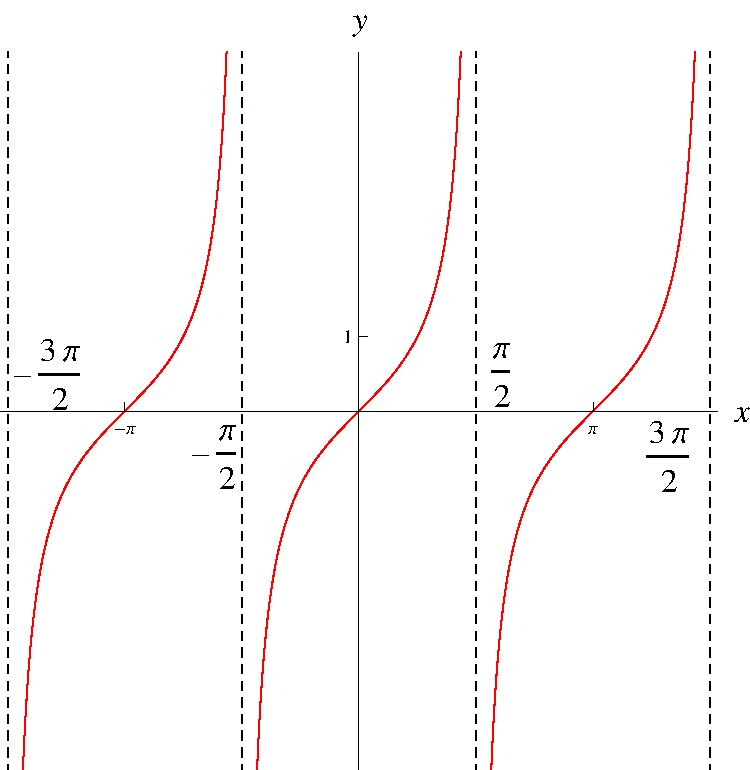
\includegraphics[width=5cm]{limits/pictures/graph-tan.pdf}

\abovedisplayskip=0pt
\belowdisplayskip=-15pt
\abovedisplayshortskip=0pt
\belowdisplayshortskip=0pt
\begin{align*}
\alertNoH{ 8-9}{\lim_{x\to \frac{\pi}{2}^+}\tan x} & \alertNoH{ 8-9}{=} \fcAnswer{9}{-\infty} \\
\alertNoH{ 10-11}{\lim_{x\to \frac{\pi}{2}^-}\tan x} & \alertNoH{ 10-11}{=} \fcAnswer{11}{\infty} \\
\alertNoH{ 12-13}{\lim_{x\to \frac{\pi}{2}}\tan x} & \alertNoH{ 12-13}{=} \fcAnswer{13}{\text{DNE}} \\
\end{align*}
\end{columns}
\end{frame}
% end module infinite-limit-ln-tan
